\section{ AR0017GB23 }


\subsection{Meta}

    \textbf{Title:}
    Approaches to the Algorithmic Allocation of Public Resources: A Cross-disciplinary Review
    
    \begin{table}[H]
        \centering
        \begin{tabular}{|c|c|c|c|c|c|c|c|c|}
            \hline
                \textbf{Rank} & \textbf{Grasp} & \textbf{Grade} & \textbf{Type} & \textbf{Outcome} & \textbf{Domain} & \textbf{COV19} & \textbf{CoI} & \textbf{DB} \\
            \hline
                3 & 98\% & B+ & A & P & B & Yes & ?? & No \\
            \hline
        \end{tabular}
        \caption{Reference's metadata}
        \label{tab:AR0017GB23}
    \end{table}

\subsection{Summary}
    Saba Esnaashari et al. \cite{x121} rendered a quantitative analysis of the five areas of public resource scheduling. From 2020 to 2023, 75 of 1070 papers were selected. The authors focus on prioritisation and perspectives chosen to develop allocation algorithms. Using PRISMA analysis, the paper highlighted the trends and tendencies in interpretability, flexibility, ethical considerations, bias, performance, and optimisation goals in reviewed studies. The outcome of the literature review yields a low level of concern for the ethics and biases by the algorithm developers. Overall, the paper brings a crucial aspect of the optimisation algorithm development and presents it with the quantitative representation of the current state of healthcare, disaster relief, organ transplantation, homelessness, and welfare. To improve the impact, the charts' metrics can be double-checked since there are possible inconsistencies with the text. The paper is a valuable reminder of the satellite aspects of responsible research.

\subsection{Notes}
    \begin{itemize}
        \item Nash equilibrium?
        \item Article 22 of the Europeans Union's General Data Protectio Regulation (GDPR) - Algorithm Interretability;
        \item Bias evaluation;
        \item Healthcare, disaster relief, organ transplantation, homelessness, welfare;
        \item Preferred Reporting Items for Systematic Reviews and Meta-Analysis (PRISMA)
    \end{itemize}


\subsection{Reading}
    \textbf{Abstract:}
    Scheduling finite resources is a challenging multi-objective task. There is not much engagement between researchers in the field. The authors found 1070 papers which were reduced to 75 studies after the screening. There is a manority of human-centric and also multi-objective approaches. The potantial gains are promissing. Neverthelss, only third part of the studies did not consider the ethical side of the research. Therefore, the authors of this review promise to guide the policy makers. It also concerns future research. 
    
    \textbf{Objectives:}
    To overview of the existing works in the field of public resource allocation and suggest guidance for the policy makers.

    
    \textbf{Page 1 (Introduction):}
    Managing finite resources is critical aspect in economic field. AI is a promising tool to acheave an efficient public resource allocation, but it also can be biased. To retain equality and justes the new policies for AI use should be created. There is examples of publications which already focusing on this aspect of the AI technology. This review was conducted to research pros and cons of the different areas of resourse allocation. The paper intented to be useful for researchers and policy makers. Structure of the work. 
    
    \textbf{Page 2 (Methodology):}
    \underline{Identification}: some algorithm on resource allocation from viriaty of areas (2020-2023). \underline{Screening}: three rounds by six researchers reduced number of studies to 75. \underline{Metric Selection}: In parallel with the screening, technical metrics were identified and analysed.
    \begin{figure}[H]
        \centering
        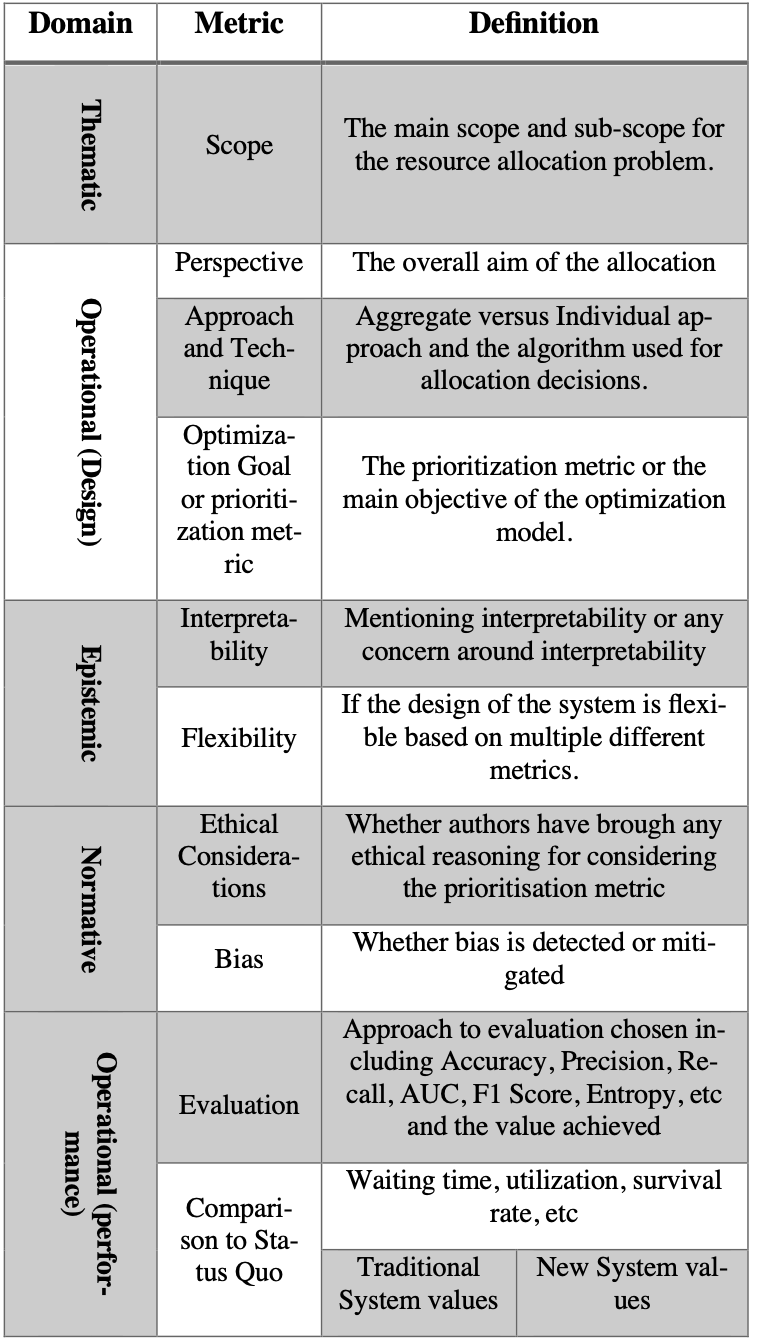
\includegraphics[width=.64\textwidth]{figures/AR0017GB23/fig1.png}
        \caption{Selected metrices in \cite{x121}.}
        \label{fig1:AR0017GB23}
    \end{figure}
    
    \textbf{Page 3 (Analysis):}
    \underline{Scope}: healthcare 71\%, disaster 14\%, oran transplantation 9\%, homelessness, and welfare. The most attention in healthcare goes to operating room and patient scheduling. Kidney transplotation is the most frequent topic in the organ transplotation. In the studies on disaster, earthquakes and maritime are mentioned the most. \underline{Perspective Human-Oriented vs. Resource-Oriented}: a solution for the same problem can be modeled using different prespectives. Nevertheless, there are also papers on the both perspectives.
    \begin{figure}[H]
        \centering
        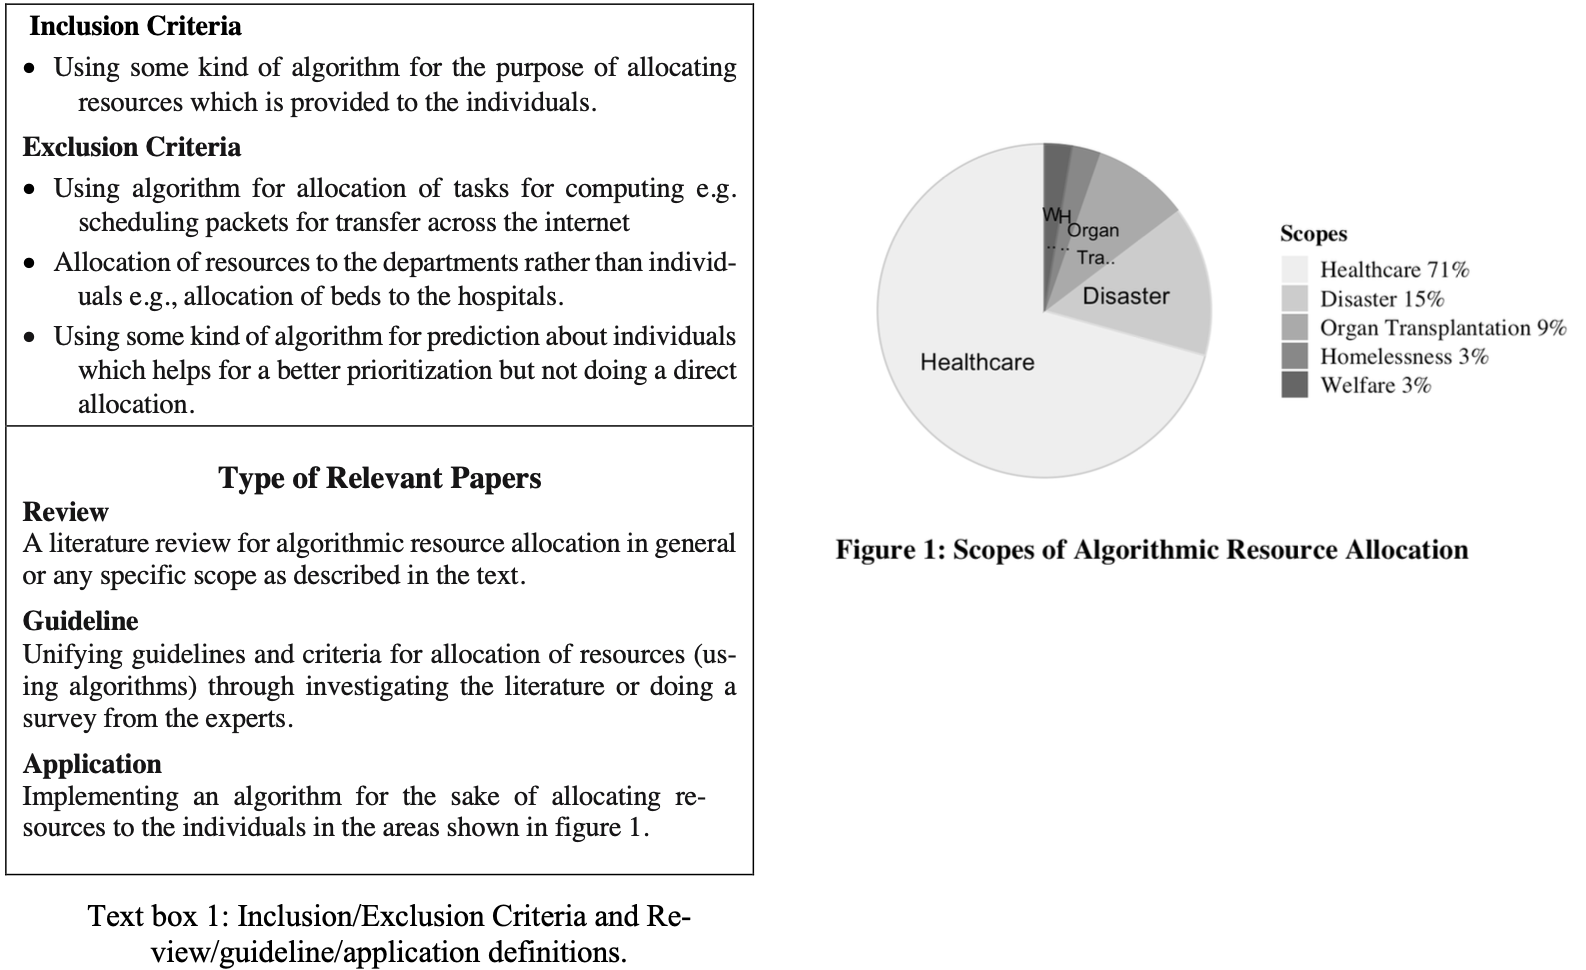
\includegraphics[width=1\textwidth]{figures/AR0017GB23/fig2.png}
        \caption{Analysis critaria from \cite{x121}.}
        \label{fig2:AR0017GB23}
    \end{figure}

    \textbf{Page 4 (Approach and Technique: Affrefate vs. Individual or Optimization vs. Prioritization):}
    Highlighting the difference between individual and aggregate points of view. the authors describe the charts shown below.
    \begin{figure}[H]
        \centering
        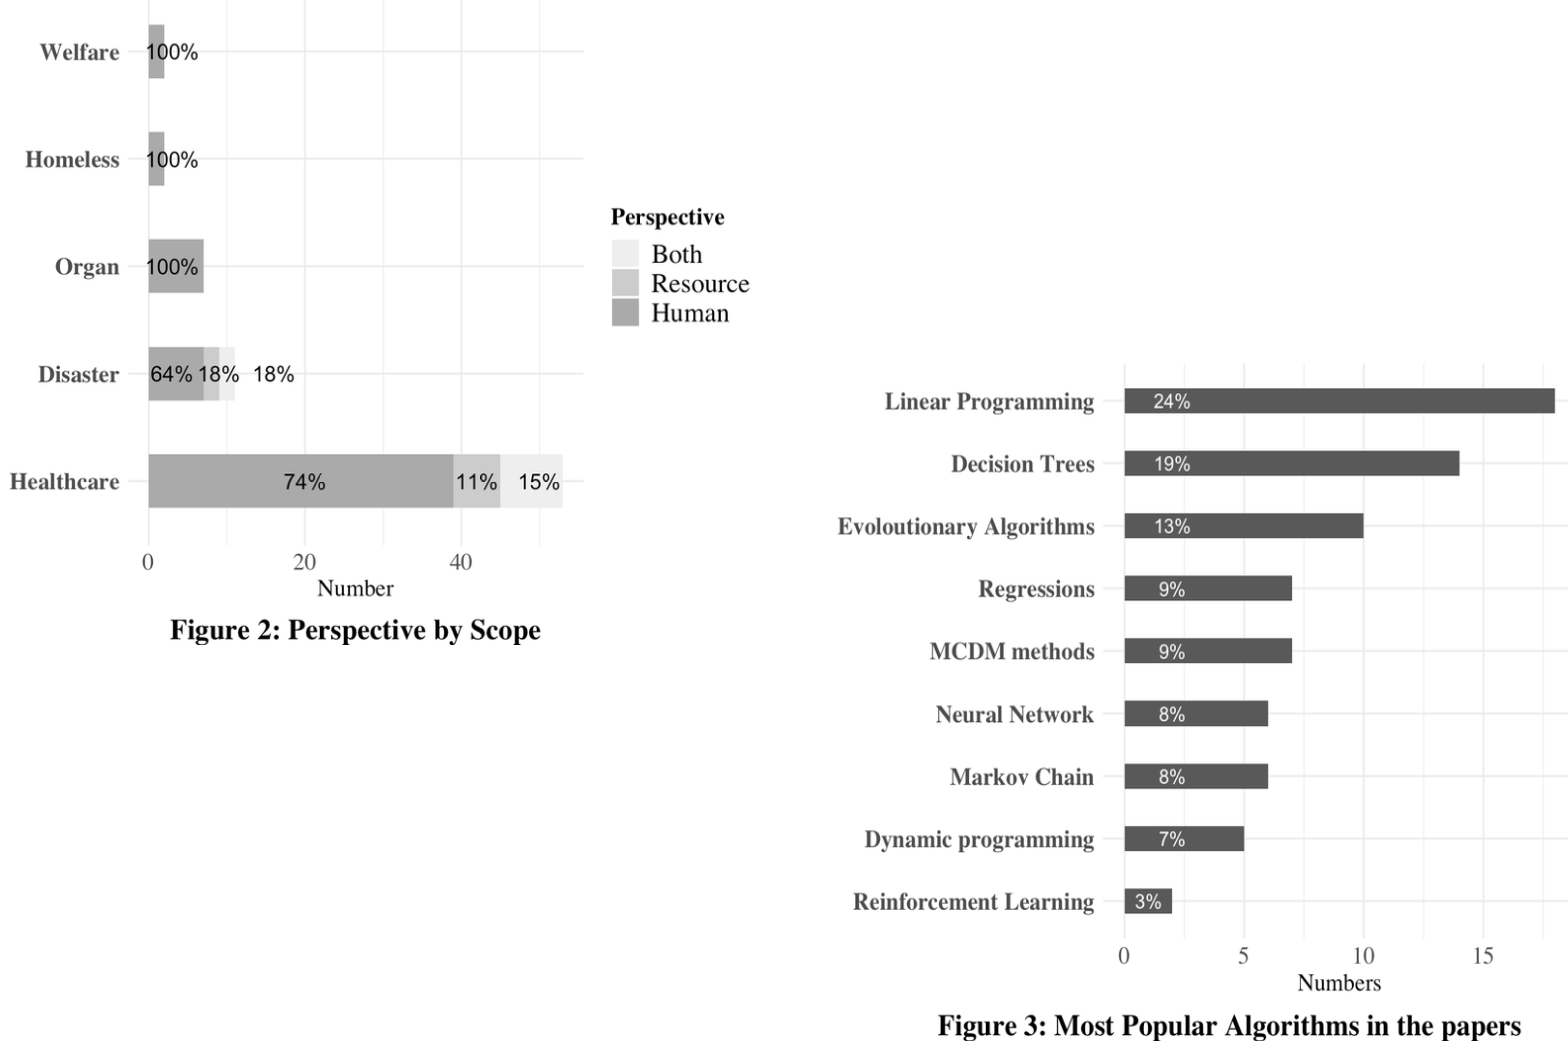
\includegraphics[width=1\textwidth]{figures/AR0017GB23/fig3.png}
        \caption{Distribution by analysis critaria from \cite{x121}.}
        \label{fig3:AR0017GB23}
    \end{figure}

    \textbf{Page 5 (Optimization goals or Prioritization metrics):}
    There are also subgroups in human-oriented group such as waiting time and preference aggregation. Healthcare and disaster sphere focuse on vulnerability critaria and organ transplantation focuses on outcome. The rest of the section describes the charts below. 
    \begin{figure}[H]
        \centering
        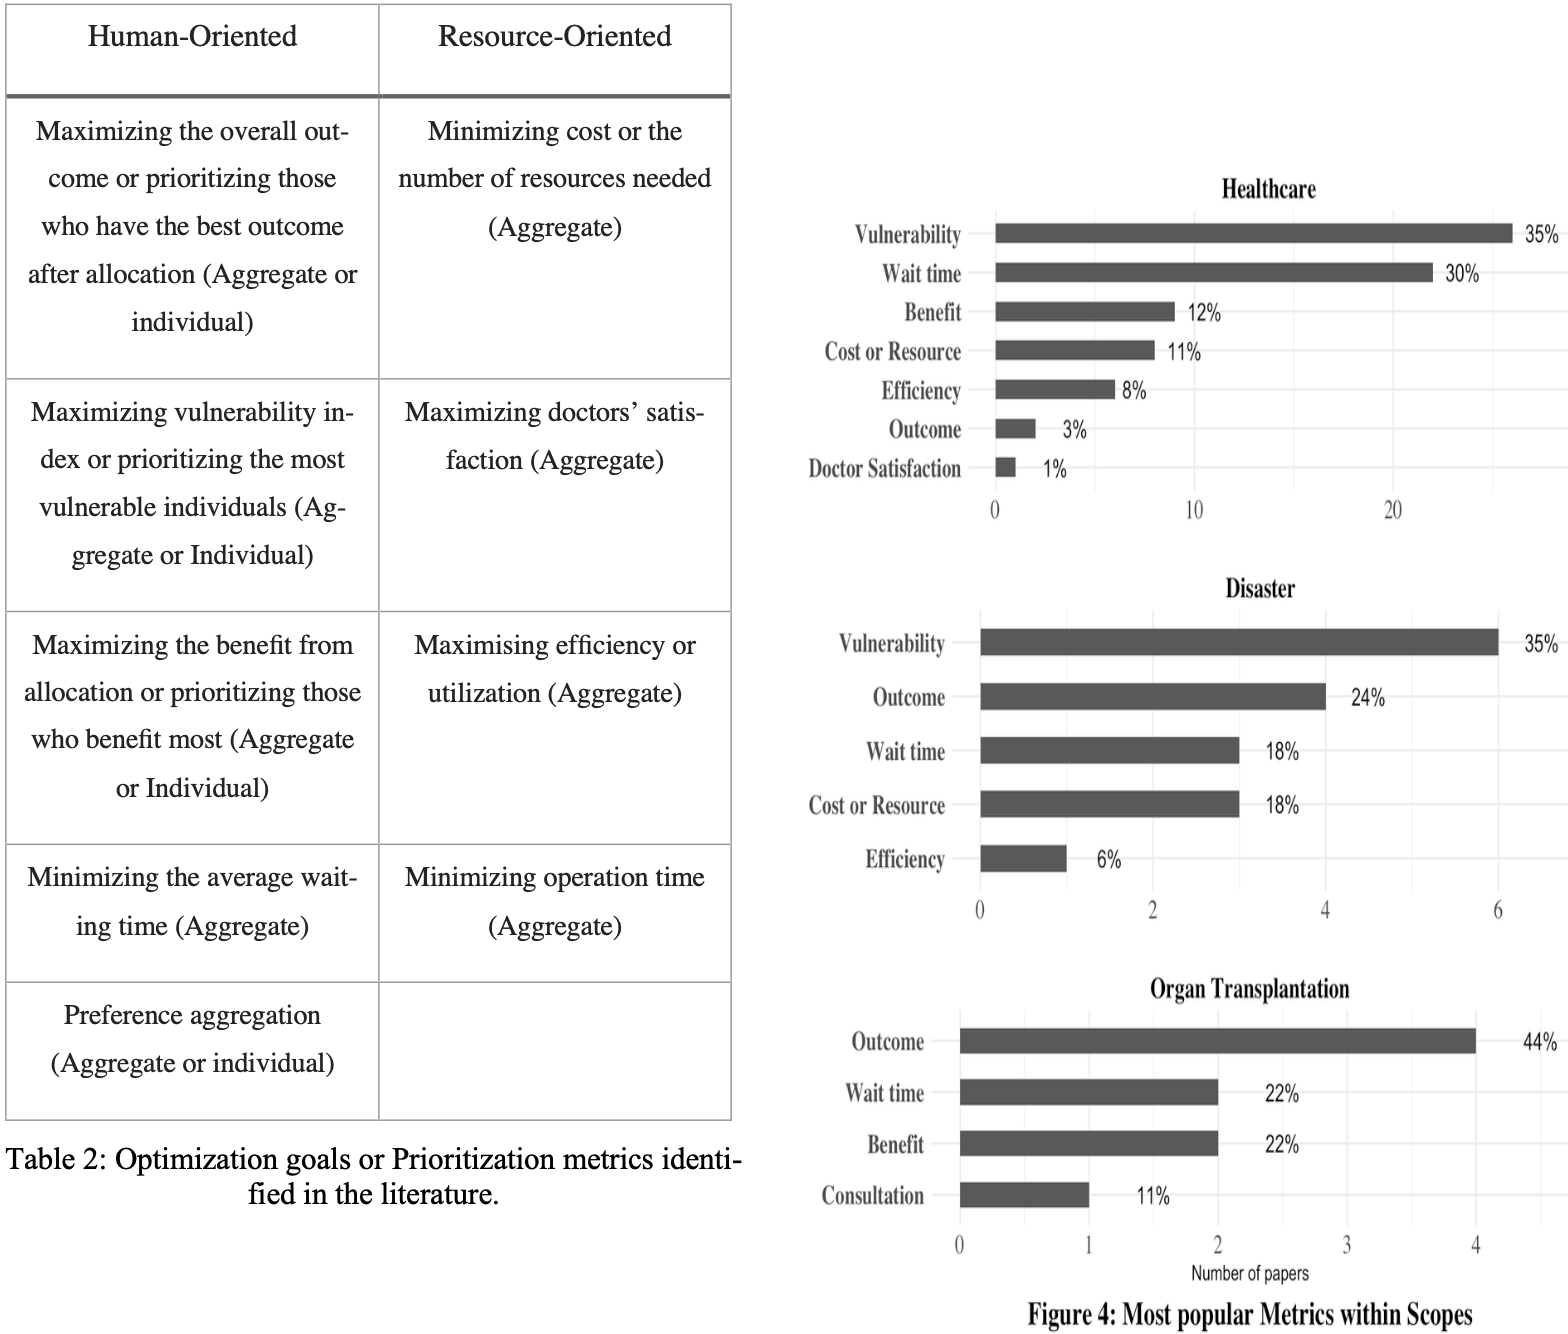
\includegraphics[width=1\textwidth]{figures/AR0017GB23/fig4.png}
        \caption{Metrix analysis from \cite{x121}.}
        \label{fig4:AR0017GB23}
    \end{figure}
    
    \textbf{Page 6 (Interpretability):}
    The regulations require from algorithm developers easy-to-understand algorithms which can come in cost of efficiensy and accuracy. Governments should be able to explain why one person is chosen over the other. The authors analysed the modern approaches focusing on the interpretability critaria and only 20\% of works are considered interpretability in their studies.
    \begin{figure}[H]
        \centering
        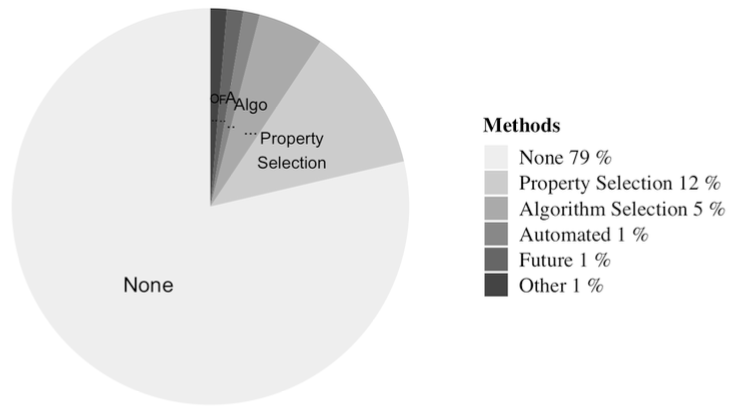
\includegraphics[width=.7\textwidth]{figures/AR0017GB23/fig5.png}
        \caption{Interpretability in the reviewed papers from \cite{x121}.}
        \label{fig5:AR0017GB23}
    \end{figure} 
    
    \textbf{Page 6 (Flexibility):} 
    to scope, time, and location changes (considered in 22\% of reviewved papers). There is a paper which balances fairness and efficiency. 
    
    \textbf{Page 7 (Ethical Considerations):}
    "Who should be prioritized and why?" This is ongoing debade in the researched areas, and only 32\% of reviewed studies reflect this concern. 
    
    \textbf{Page 7 (Bias):}
    The developed algorithms should meet "non-discrimination" by GDPR. Only 4\% of papars has tests on difining whether the proposed methods are biased. 
    
    \textbf{Page 7 (Performance) = evaluation + comparison to status quo}
    
    \textbf{Page 7 (Evaluation):}
    Machine learning evaluation metrics: accuracy, F1, precision, recall, and AUC. On average these metrics lay between 82\% and 89\% (more in appendix A2).
    
    \textbf{Page 7 (Comparison to the Status Quo):}
    the most popular objectives (with avg. improvement rates) are survival rate (20\%), waiting time (49\%), and utilization (46\%) (more in appendix A3). (reflection: the values on the charts in A3 does not exectly match the results in the text).

    \textbf{Page 8 (Conclusion and Discussion):}
    The authors repeat and summarise everything said in the body of the paper: 75 reviewed papers, 5 categories, humna- vs. resource-oriented approaches, and personal- vs aggregate-oriented approaches. Resouce oriented perspective in healthcare and welfare holds open the ehical questions. The improved efficiency of the algorithms looks promising but the issues related to bias and interpretability requires more research and deeper understanding. The topic of resouce allocation sky-rocketted for the recent years. The authors want this paper to be usefull for researchers and policy desicion-makers.